\documentclass[a4paper]{article}
\usepackage[14pt]{extsizes} % для того чтобы задать нестандартный 14-ый размер шрифта
\usepackage[left=1.5cm,right=1.5cm,top=2cm,bottom=2cm]{geometry}
\usepackage{multirow}
\usepackage{parallel}
\usepackage {graphicx}
\usepackage{multicol}
\usepackage[utf8x]{inputenc} % указать кодировку русского текста
\usepackage[russian]{babel} % указать, что язык текста - русский
\usepackage{fancyhdr}
\pagestyle{fancy}
\usepackage{graphicx}
\graphicspath{{pictures/}}
\DeclareGraphicsExtensions{.pdf,.png,.jpg, .jpeg}
\usepackage{tocloft}
\usepackage{wrapfig}
\usepackage{tikz}

\usepackage{enumitem}
\setlist[enumerate,itemize]{leftmargin=0pt,itemindent=2.7em}
\renewcommand{\cftsecleader}{\cftdotfill{\cftdotsep}}
\begin{document} 
\large
\noindent \textbf{Интерференция от двух независимых источников}\\
\\
\normalsize
\line(1,0){18cm}\\
\\
\small
Пусть имеется два независимых точечных источника излучения. Каждый из них излучает, соответственно, гармонические волны 
\begin{equation}
E_1 = E_{10}\cos(\omega_1 t - k_1l_1 + \phi_1) \; , \; \; E_1 = E_{20}\cos(\omega_2 t - k_2l_2 + \phi_2)
\end{equation}
до некоторой точки экрана - точки А.\\
\begin{center}
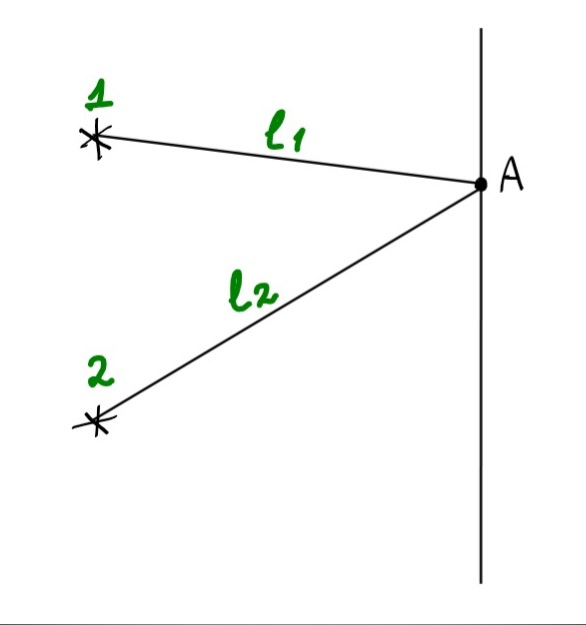
\includegraphics[width=5cm]{t1}
\end{center}
Суммарное поле в точке А определяется по принципу суперпозиции двух полей.\\
Мы знаем, что интенсивность $I \propto <|E|^2>$, поэтому:

$$I \propto <E_{10}^2\cos^2(\omega_1 t - k_1l_1 + \phi_1)> + <E_{20}^2\cos^2(\omega_2 t - k_2l_2 + \phi_2)> + $$
$$ + 2(E_{10} + E_{20})<\cos(\omega_1 t - k_1l_1 + \phi_1)><\cos(\omega_2 t - k_2l_2 + \phi_2)> = \frac{E_{10}^2}{2} + \frac{E_{20}^2}{2} + $$ $$+2(E_{10} + E_{20})<\cos(\omega_1 t - k_1l_1 + \phi_1)><\cos(\omega_2 t - k_2l_2 + \phi_2)>$$ 
\\
Воспользуемся тригонометрической формулой $\cos \alpha \cdot \cos \beta = 0,5(\cos (\alpha - \beta) \cos (\alpha + \beta))$
Так как $\cos ((\omega_1 + \omega_2)t)$ - величина очень большая ($\omega$ порядка $10^15$ $c^{-1}$), то при усреднении здесь получится ноль, поэтому от третьего слагаемого останется:
$$(E_{10} + E_{20})<\cos((\omega_1 - \omega_2)t - k_1l_1 + k_2l_2 + \delta \phi)>$$
Запишем теперь это по-другому:
\begin{equation}
I = I_1 + I_2 + I_{12}, \; \; I_{12} = (E_{10} + E_{20})<\cos((\omega_1 - \omega_2)t - k_1l_1 + k_2l_2 + \delta \phi)>
\label{simple}
\end{equation}
где $I_{12}$ - вклад в интенсивность от интерференции двух волн!\\
Таким образом, чтобы этот вклад не был нулевым, должно выполняться три условия:
\begin{enumerate}
\item $\omega_1 = \omega_2$, сл-но $k_1 = k_2$
\item $\delta \phi = const$
\item $(E_{10}, E_{20})\neq 0$
\end{enumerate}
Разберем каждый из этих случаев:
\begin{enumerate}
\item $\omega_1 = \omega_2$\\
Это значит, что волны должны иметь одинаковую частоту.\\
\item $\delta \phi = const$\\
То есть волны должны быть когерентны. В то же время волны от двух независимых источников некогерентны, поэтому разность их фаз, стоящая под косинусом, будет зависеть от времени, следовательно, при усреднении даст ноль и интерференции не будет.
\end{enumerate}
Таким образом, главный камень преткновения в излучении двух независимых источников - это их некогерентность, начальные фазы каждой из волн меняются случайным образом, из-за этого меняется случайным образом разность фаз результирующих колебаний, поэтому при усреднении она даст ноль и интерференции не будет.
\end{document}